%\documentclass[25pt, a3paper]{tikzposter}
\documentclass{tikzposter}
\usepackage[utf8]{inputenc}
\usepackage[backend=bibtex]{biblatex}
\addbibresource{cs698o_proj.bib}

\title{CS698O Project: Knowledge Distillation and its Variations}
\author{Sandipan Mandal, Teekam Chand Mandan}
\date{\today}
\institute{Indian Institute of Technology Kanpur}

\usepackage{blindtext}
\usepackage{comment}
\usetheme{Board}

\begin{document}
\fontsize{30}{50}
\maketitle

\block[bodywidthscale=.5]
{Sample Block}{Text\\Text\\Text Text}
\begin{columns}
\column{1.0}
\block{Introduction}{In this project, we have implemented Knowledge Distillation(KD) from \cite{hinton2015distilling} and tried some variations of it. We evaluated the performance of KD on MNIST, notMNIST and SVHN datasets. Finally we have also implemented the paper Fitnets : Hints for Thin Deep Nets\cite{romero2014fitnets} and evaluated it on MNIST dataset.}
\end{columns}

\begin{columns}
    \column{0.5}
    \block{Knowledge Distillation}{In KD, we train a large teacher network \textbf{T}. We train our smaller student network \textbf{S} using a composite loss function consisting of two terms, one optimizing to improve label prediction accuracy, other to match pre-softmax logits with teacher \textbf{T}. Loss function is given by : $$L(W_S) = H(y_{true}, P_S) + \lambda H(P_T^{\tau}, P_S^{\tau})$$ where $H$ is the cross-entropy loss function, $y_{true}$ is the true label, $P_S$ is the softmax output of \textbf{S}, $P_T^{\tau}, P_S^{\tau}$ are respectively softmax output of \textbf{T} and \textbf{S} after dividing the corresponding logits by $\tau$.  }
    

    \column{0.5}
    \block{Basic Adversarial Knowledge Distillation}{Here, we train a large teacher network \textbf{T} and smaller student network \textbf{S}. Using \textbf{T} and \textbf{S}, we train a discriinator network \textbf{D}, which can distinguish if a logit is constructed from \textbf{T} or \textbf{S}. We train our final student network \textbf{S} using a composite loss function consisting of two terms, one optimizing to improve label prediction accuracy, other to match pre-softmax logits with teacher \textbf{T}. The only difference here is that the logit matching is done adversarially using \textbf{D}. The loss function is given by : $$L(W_S) = \alpha H(y_{true}, P_S) - \beta L_{class}(a_S = )$$ where $H$ is the cross-entropy loss function, $y_{true}$ is the true label, $P_S$ is the softmax output of \textbf{S}, $P_T^{\tau}, P_S^{\tau}$ are respectively softmax output of \textbf{T} and \textbf{S} after dividing the corresponding logits by $\tau$.  }
\end{columns}

\begin{columns}
    \column{0.5}
    \block{Knowledge Distillation using GANs/WGANs}{In KD, we train a large teacher network \textbf{T}. We train our smaller student network \textbf{S} using a composite loss function consisting of two terms, one optimizing to improve label prediction accuracy, other to match pre-softmax logits with teacher \textbf{T}. Loss function is given by : $$L(W_S) = H(y_{true}, P_S) + \lambda H(P_T^{\tau}, P_S^{\tau})$$ where $H$ is the cross-entropy loss function, $y_{true}$ is the true label, $P_S$ is the softmax output of \textbf{S}, $P_T^{\tau}, P_S^{\tau}$ are respectively softmax output of \textbf{T} and \textbf{S} after dividing the corresponding logits by $\tau$.  }
    

    \column{0.5}
    \block{}{}
\end{columns}

%\begin{columns}
%    \column{1}
%    \block{The model architecture (from the paper)}
%    {
%        \begin{tikzfigure}
%            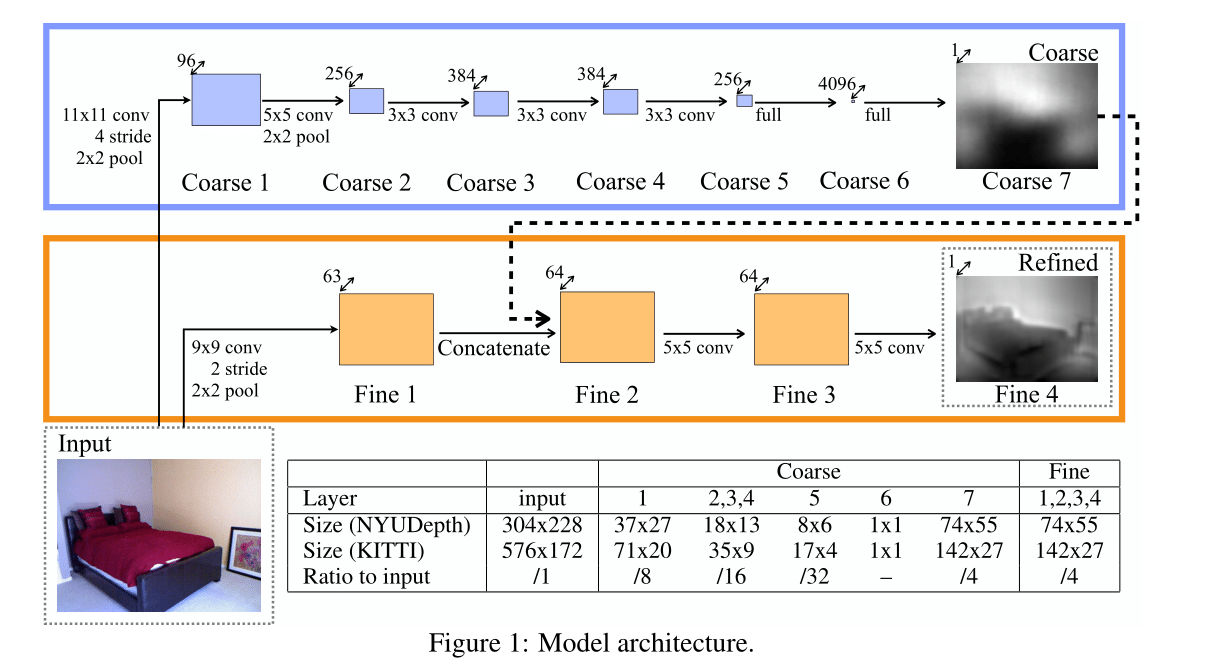
\includegraphics[width=0.8\textwidth]{images/model.png}
%        \end{tikzfigure}
%    }
%\end{columns}


\block{References}{\printbibliography[heading=none]}

\end{document}

